\chapter{Describing Fission Using Nuclear Density Functional Theory}\label{chap:Model}

%(Nicolas gave a good annotated presentation in 2017 that describes some of the philosophy, as well as some of the outstanding challenges of spontaneous fission in an adiabatic framework: \verb|https://t2.lanl.gov/fiesta2017/school/Schunck_NotesSlides.pdf|)

Today there are two microscopic frameworks in which to study fission: time-dependent and static (time-independent). Time-dependent approaches evolve the system in real-time. Since fission is an inherently time-dependent process, these methods offer great insight into the fission process and the characteristics of the fragments, especially kinetic and excitation energies~\cite{Scamps2018, Scamps2015a, Simenel2014, Grineviciute2018, Umar2010}. However, they can only treat a single event at a time and are quite expensive, making them impractical for fission yield predictions. Despite efforts such as~\cite{Scamps2015, Bulgac2018}, there is currently no way to obtain a full yield distribution in a time-dependent framework.

More important to the present discussion, though, is the fact that time-dependent approaches are totally unsuited to spontaneous fission calculations. Spontaneous fission is fundamentally a quantum tunneling process, and at present there is no tunneling mechanism within time-dependent approaches. Furthermore, time-dependent computations tend to break down after too many time steps. Even if the tunneling problem was solved, this approach would still fail for any nucleus with a reasonably-long lifetime (compared to a typical time step size around ${\sim}10^{-24}$sec).

On the other hand, static approaches assume that collective motions of the nucleus are slow compared to the motion of the intrinsic particles, and therefore that collective and intrinsic degrees of freedom can be decoupled. This assumption, called the adiabatic approximation, is supported by experimental evidence which suggests a characteristic timescale for fission (from saddle to scission, the point at which the neck snaps) of ${\sim}10^{-20}-10^{-18}$sec, compared to typical nuclear timescales on the order of ${\sim}10^{-22}$sec (see~\cite{Jacquet2009} for a review of fission timescale experiments). The validity of the adiabatic assumption was further discussed for fission and other nuclear processes in~\cite{Nazarewicz1993}.

The assumption of adiabaticity justifies the creation of a potential energy surface (PES) in some space of collective shape coordinates, and the dynamics of fission are then described as trajectories across the PES. Quantum tunneling pops out in a fairly natural way in this formalism, and half-life estimates follow. Calculating the kinetic and excitation energies in this framework is straightforward in principle, but in practice it is extremely sensitive to the scission configurations used~\cite{Younes2011}. However, the static approach is well-suited to estimating fission yields.

%Adiabaticity: For fusion reactions, N,Z equilibrium reached in ${\sim}10^{-21}$ seconds, then energy/thermal equilibrium in a similar time scale, then finally mass equilibrium in ${\sim}10^{-19}$ - Yuri has a slide with these time scales from his talk Monday. By comparison, what is an appropriate timescale for collective motion? I suppose that is nucleus-dependent

In an effort to be as self-consistent as possible, the PES is computed in the framework of nuclear DFT, which combines the Hartree-Fock-Bogoliubov (HFB) variational approximation to the energy with a many-body method inspired by Kohn-Sham DFT. An overview of this self-consistent mean-field framework is described below, followed by a description of the dynamical calculations which are used to calculate fission yields.

\section{Nuclear density functional theory}
Since nuclei are quantum systems, they can in principle be described using the Schr\"{o}dinger equation. In practice, however, one finds this type of description difficult or impossible, for two reasons:

\begin{itemize}
\item In order to use the Schr\"{o}dinger equation, one needs to describe the interaction between particles, in this case protons and neutrons. However, protons and neutrons are made up of quarks and gluons, which interact via the strong nuclear force. Consequently, an analytic expression for the nucleon-nucleon interaction (analogous to the $\frac{1}{r}$ form of the Coulomb interaction) is not available.
\item Even if an interaction was known, nuclei are large systems made up of many protons and neutrons. Solving the Schr\"{o}dinger equation directly quickly becomes computationally intractable as the number of nucleons increases.
\end{itemize}

Nuclear density functional theory is one of several methods which has been developed to address these challenges. It is particularly useful for heavy nuclei, where more precise \textit{ab initio} methods become prohibitively expensive.

\subsection{Density functional theory}\label{sect:DFT}
Nuclear DFT is rooted in the Hohenberg-Kohn theorems~\cite{Hohenberg1964}, which follow.

Suppose a system is described in second quantization by a set of creation and annihilation operators $c_i, c_i^\dagger$ which act on the vacuum state $\ket{\psi_0}$ to create single-particle states $c_i^\dagger\ket{\psi_0}$. Define the density: $\rho_{ij} = \expval{c_j^\dagger c_i}{\psi_0}$. The first Hohenberg-Kohn theorem states that the energy of the system is a uniquely-defined functional of the density. That means that if a system of interacting particles and a system of noninteracting particles give the same density, the energy of those systems will be the same. This gives one the freedom to describe a system using a mean-field method instead of having to describe the pairwise interactions between each and every particle - a huge simplification!

The second Hohenberg-Kohn theorem states that the functional which gives the energy of the system will give the ground state energy if, and only if, it acts on the true ground state density. Thus, given a particular functional, one can vary the input density to minimize the total energy and be assured that we are approaching the ground state energy of the system. A variational prescription was subsequently proposed by Kohn and Sham in~\cite{Kohn1965}, but because of the importance of pairing correlations in nuclear dynamics, we will instead use the HFB variational method. HFB mirrors the spirit of Kohn-Sham but with the inclusion of an additional pair density $\kappa_{ij} = \expval{c_jc_i}{\psi_0}$, which can be thought of as a coupling between the vacuum state and a state with two particles (in states $i$ and $j$). The pair density $\kappa$ is combined with the single-particle density $\rho$ to form a generalized density

\begin{equation}
\mathcal{R} = \left(\begin{array}{cc}
\rho & \kappa \\
-\kappa^* & 1-\rho^*
\end{array}\right)
\end{equation}

In coordinate space, the density matrix $\rho$ and the pair tensor $\kappa$ take the form

\begin{align}
\rho(\vec{r},\vec{r}') &= \expval{c_{\vec{r}'}^\dagger c_{\vec{r}}}{\psi_0} \\
\kappa(\vec{r},\vec{r}') &= \expval{c_{\vec{r}'} c_{\vec{r}}}{\psi_0}
\end{align}

\noindent Note that in nuclei, there are two $\rho$s and two $\kappa$s: one set for describing neutrons and another for protons.

The next step is to find the correct energy density functional. Unfortunately, neither the Hohenberg-Kohn theorems nor the Kohn-Sham method specified how this is to be done. Typically at this point the total energy is divided into a sum of several contributions, which can each be treated individually:

\begin{equation}
E(\rho, \kappa) = E_{kin} + E_{Coul} + E_{nuc} + E_{pair}
%E(\rho, \kappa) = \int d^3\vec{r}\sum_{t=0,1}\mathcal{H}_t = \int d^3\vec{r}\left(\mathcal{H}_{kin} + \mathcal{H}_{nuc} + \mathcal{H}_{Coul, dir} + \mathcal{H}_{Coul, exch} + \mathcal{H}_{pair}\right)
\end{equation}

\noindent where $E_{kin}$ is the kinetic energy term, $E_{Coul}$ contains the Coulomb interaction between protons, $E_{nuc}$ is a nucleon-nucleon interaction term, and $E_{pair}$ describes the tendency of nucleons to form pairs, which would otherwise be smeared out in non-interacting mean-field models. Portions of the energy density functional corresponding to each of these terms are described below.

\subsubsection{Kinetic energy term}

Defining the kinetic density $\tau_\alpha = \left.\nabla\cdot\nabla'\rho_\alpha(\vec{r},\vec{r}')\right|_{\vec{r}=\vec{r}'}$, $\alpha=p,n$, the kinetic energy contribution is

\begin{equation}
E_{kin} = \frac{\hbar^2}{2m} \left(1-\frac{1}{A}\right) \int d^3\vec{r} \left(\tau_n(\vec{r}) + \tau_p(\vec{r}) \right)
\end{equation}

\noindent The $\left(1-\frac{1}{A}\right)$ term is a simple, approximate center-of-mass correction.

\subsubsection{Coulomb interaction term}
The Coulomb interaction between protons is divided into a direct term and an exchange term, which is related to the antisymmetry of fermion wavefunctions:

\begin{align}
E_{Coul} &= E_{Coul, dir} + E_{Coul, exch} \\
E_{Coul, dir}& = \frac{e^2}{2} \int d^3\vec{r}_1 d^3\vec{r}_2 \frac{\rho_p(\vec{r}_1)\rho_p(\vec{r}_2)}{\abs{\vec{r}_1-\vec{r}_2}} \\
E_{Coul, exch} &= \frac{e^2}{2} \int d^3\vec{r}_1 d^3\vec{r}_2 \frac{\rho_p(\vec{r}_2,\vec{r}_1)\rho_p(\vec{r}_1,\vec{r}_2)}{\abs{\vec{r}_1-\vec{r}_2}}
\end{align}

Often the exchange term is computed in the Slater approximation~\cite{Slater1951, TitinSchnaider1974}:

\begin{equation}
E_{Coul, exch} \approx -\frac{3e^2}{4} \left(\frac{3}{\pi}\right)^\frac{1}{3} \int d^3\vec{r} \rho_p^\frac{4}{3}(\vec{r})
\end{equation}

\subsubsection{Nuclear interaction term}
Describing the interaction between nucleons $E_{nuc}$ (and to a lesser extent, $E_{pair}$) continues to be an active area of research in nuclear theory today~\cite{Machleidt2011,Machleidt2016,Epelbaum2009,Detmold2015,Stroberg2019}. For nuclear DFT, the most commonly-used interactions belong to the Skyrme, Gogny, or covariant family of functionals (each of which is discussed in~\cite{Bender2003}). We will primarily be using Skyrme functionals, which can be written as a sum of both time-even and time-odd terms:

\begin{align}
E_{Skyrme} &= \int d^3\vec{r} \sum_{t=0,1} \left( \mathcal{H}^{even}_t + \mathcal{H}^{odd}_t \right)\\
\mathcal{H}^{even}_t &= C^\rho_t\rho_t^2 + C_t^{\Delta\rho}\rho_t\Delta\rho_t + C^\tau_t\rho_t\tau_t + C^J_t\mathsf{J}^2_t + C^{\nabla J}_t\rho_t\nabla\cdot\vec{J}_t \\
\mathcal{H}^{odd}_t &= C^s_t \vec{s}_t^2 + C_t^{\Delta s}\vec{s}_t\Delta\vec{s}_t + C^T_t\vec{s}_t\cdot\vec{T}_t + C^j_t\mathsf{j}^2_t + C^{\nabla j}_t\vec{s}_t\cdot(\nabla\times\vec{j}_t)
\end{align}

\noindent where $\tau_t$ is the kinetic energy density; $\mathsf{J}_t$ is the spin current density, with vector part given by $\vec{J}_{\kappa,t} = \sum_{\mu\nu}\epsilon_{\mu\nu\kappa}\mathsf{J}_{\mu\nu,t}$; $\vec{s}_t$ is the spin density, $\vec{T}_t$ is the spin kinetic density; and $\vec{j}_t$ is the momentum density (to see how these are each related to $\rho$, see, e.g.,~\cite{Bender2003}). The index $t=0(1)$ refers to isoscalar(isovector) energy densities, e.g., $\rho_0 = \rho_n + \rho_p$ ($\rho_1 = \rho_n - \rho_p$). Note that $\mathcal{H}^{even}_t$ depends only on time-even densities (and likewise for $\mathcal{H}^{odd}_t$).

Since this interaction is phenomenological, based on a zero-range contact interaction between nucleons, the coefficients are adjustable. There are dozens of Skyrme parameterizations on the market, each one optimized to a particular observable or set of observables. The parameter sets SkM*~\cite{Bartel1982} and UNEDF1~\cite{Kortelainen2012} (along with its sister, {\hfb}~\cite{Schunck2015}) are optimized to datasets which include fission data, making them suitable for fission calculations.

\subsubsection{Pairing interaction term}
The mean field approximation fails to take into account some correlations between nucleons, especially those which occupy similar states. Nucleons in nearby states (for example, with equivalent orbital quantum numbers but opposite spins) have a tendency to form pairs, similar to BCS superconductivity or $^3$He superfluidity. To account for this phenomenon, we use a density-dependent pairing interaction:

\begin{equation}
E_{pair} = V_0 \int d^3\vec{r} \left( 1-\left(\frac{\rho(\vec{r})}{\rho_0}\right)^\alpha \right)
\end{equation}

\noindent As with the nuclear interaction term, the pairing interaction contains several adjustable parameters $V_0, \alpha,$ and $\rho_0$. $\rho_0$ determines whether pairing takes place more within the volume ($\rho_0\rightarrow\infty$), around the surface ($\rho_0\approx0.16$ fm$^{-3}$), or somewhere in between. The exponent $\alpha$ affects the formation of surface effects, such as neutron skins and halos, but is usually set to $\alpha=1$. The pairing strength $V_0$ may be adjusted to odd-even mass differences.

\subsection{Hartree-Fock-Bogoliubov method}
\subsubsection{Bogoliubov transformation}

In anticipation of the HFB formalism below, we define the so-called Bogoliubov transformation. The fundamental entities in the Bogoliubov transformed basis are `quasiparticle' states, defined by quasiparticle creation and annihilation operators acting on a quasiparticle vacuum state $\ket{\Phi_0}$ (in contrast to the single particle operators from before). The quasiparticle creation and annihilation operators are given by

\begin{align}
\beta_\mu &= \sum_i U^*_{i\mu}c_i + \sum_i V^*_{i\mu}c_i^\dagger \\
\beta_\mu^\dagger &= \sum_i U_{i\mu}c_i^\dagger + \sum_i V_{i\mu}c_i
\end{align}

\noindent or in block matrix notation,

\begin{equation}
\left(\begin{array}{c} \beta \\ \beta^\dagger\end{array}\right) = 
\left(\begin{array}{cc} U^\dagger & V^\dagger \\ V^T & U^T \end{array}\right)
\left(\begin{array}{c} c \\ c^\dagger\end{array}\right)
\equiv \mathcal{W}^\dagger \left(\begin{array}{c} c \\ c^\dagger\end{array}\right)
\end{equation}

\noindent where the transformation matrix $\mathcal{W}$ must be unitary to ensure that $\beta, \beta^\dagger$ obey the fermion commutation relations~\cite{Ring1980}. In this transformed basis, the density matrix takes the form 

\begin{equation}
\mathsf{R} = \mathcal{W}^\dagger\mathcal{R}\mathcal{W} = 
\left(\begin{array}{cc}
\expval{\beta_\mu^\dagger \beta_\nu}{\Phi_0} & \expval{\beta_\mu \beta_\nu}{\Phi_0} \\
\expval{\beta_\mu^\dagger \beta_\nu^\dagger}{\Phi_0} & \expval{\beta_\mu \beta_\nu^\dagger}{\Phi_0}
\end{array}\right) = 
\left(\begin{array}{cc}
0 & 0 \\
0 & I_N
\end{array}\right)
\end{equation}

%In general, $E$ is a functional of the generalized density $\mathcal{R}$.

\subsubsection{HFB equations}

The ground state configuration of the system with a particular energy density functional is described by the density $\mathcal{R}$ which minimizes $E(\mathcal{R})$. We can find this solution through the variational principle. We minimize the energy with respect to the generalized density, subject to the constraint that $\mathcal{R}^2=\mathcal{R}$ - or in other words, subject to the constraint that the state remains a quasiparticle vacuum. Defining the HFB Hamiltonian $\mathcal{H}_{ba} \equiv 2 \partial E/\partial \mathcal{R}_{ab}$, this variation leads to the result $\left[\mathcal{H},\mathcal{R}\right]=0$, which is called the Hartree-Fock-Bogoliubov equation.

The HFB equation is not typically solved in its commutator form, but is rather recast in the following way: Recalling that two Hermitian operators whose commutator is zero can be simultaneously diagonalized, we choose to diagonalize $\mathcal{H}$ using the same Bogoliubov transformation $W$ which diagonalizes $\mathcal{R}$:

\begin{equation}
W^\dagger \mathcal{H} W \equiv \mathcal{E} \qquad\mathrm{or}\qquad \mathcal{H}W = W\mathcal{E}
\end{equation}

\noindent where

\begin{equation}
\mathcal{E} = \left(\begin{array}{cc}
E_\mu & 0 \\
0 & -E_\mu
\end{array}\right)
\end{equation}

\noindent is a matrix of quasiparticle energies. In this form, the problem can then be solved iteratively:
\begin{enumerate}
	\setlength\itemsep{-2em}
	\item Choose some ansatz to estimate the density\\
	\item Construct the Hamiltonian density $\mathcal{H}$\\
	\item Solve the eigenvalue problem \label{hfb_iteration}\\
	\item Extract the corresponding densities corresponding to the eigenfunctions (since the densities are related to $\mathcal{W}$)\\
	\item Update $\mathcal{H}$ \\
	\item Repeat starting from~\ref{hfb_iteration} until some predetermined convergence criterion is met
\end{enumerate}

% https://ocw.mit.edu/courses/physics/8-04-quantum-physics-i-spring-2013/study-materials/MIT8_04S13_OnCommEigenbas.pdf

Often, one will want to minimize the energy of the system subject to a particular constraint. Constraints can be introduced via the method of Lagrange multipliers. Some common examples might be the shape of the nucleus, where a particular multipole moment might be constrained to the value $\bar{Q}_{\lambda\mu}$

\begin{equation}
E' = E - \sum_{\lambda\mu} C_{\lambda\mu} \left(\expval{\hat{Q}_{\lambda\mu}} - \bar{Q}_{\lambda\mu}\right)^2
\end{equation}

\noindent Since the Bogoliubov transformation breaks particle number symmetry, another possible constraint might be this simple form of particle number restoration (more sophisticated forms, such as Lipkin-Nogami~\cite{Lipkin1960, Nogami1964, Pradhan1973, Flocard1997}, also exist):

\begin{equation}
E' = E - \lambda_n \expval{\hat{N}_n} - \lambda_p \expval{\hat{N}_p}
\end{equation}

\noindent where $\lambda_\alpha$ is determined later by the condition that $\expval{\hat{N}_\alpha} = N_\alpha$. In these casesS, the Hamiltonian $E$ would be replaced by with the Routhian $E'$ before variation. % Discuss PAV and VAP? Only if requested

\subsection{Nucleon localization function}\label{sect:locali}
The major advantage DFT offers of microscopic-macroscopic models is a direct link to the underlying many-body system. This can be visualized using the nucleon localization function (NLF), introduced in~\cite{Reinhard2011,Zhang2016}. The NLF is defined using the single particle density in the following way (with q=isospin and $\sigma$=spin/signature quantum number):

\begin{equation}
\mathcal{C}_{q\sigma} = \left[1+\left(\frac{\tau_{q\sigma}\rho_{q\sigma}-\frac{1}{4}|\nabla\rho_{q\sigma}|^2-\mathbf{j}^2_{q\sigma}}{\rho_{q\sigma}\tau_{q\sigma}^{TF}}\right)^2\right]
\end{equation}

\noindent where $\tau_{q\sigma}^{TF}=\frac{3}{5}(6\pi^2)^\frac{2}{3}\rho_{q\sigma}^\frac{5}{3}$. A localization value $\mathcal{C} \approx 1$ means that nucleons are well-localized; that is, the probability of finding two nucleons of equal spin and isospin in the same spatial region is low. A value of $\mathcal{C}=\frac{1}{2}$ corresponds to a Fermi gas of nucleons, as found in nuclear matter.

\begin{figure}
	\centering
	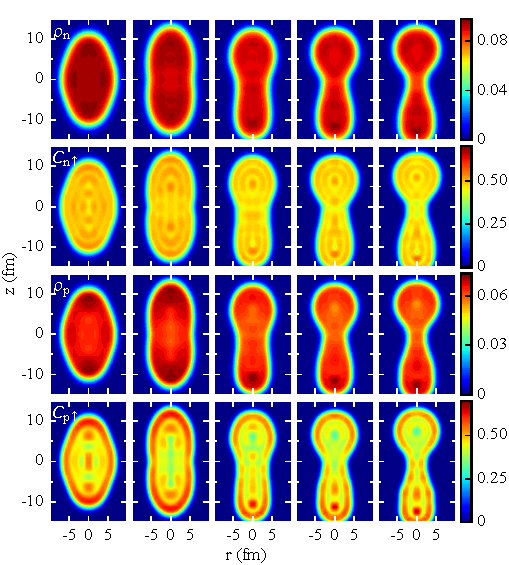
\includegraphics[width=0.5\linewidth]{TeX_files/methods_locali}
	\caption[Nucleonic densities (in nucleons/fm$^3$) and spatial localizations for $^{240}Pu$]{Nucleonic densities (in nucleons/fm$^3$) and spatial localizations for $^{240}Pu$ at several configurations along the most-probable path to fission. Source:~\cite{Zhang2016}}
	\label{fig:methodslocali}
\end{figure}

As demonstrated in Figure~\ref{fig:methodslocali}, the NLF offers greater insight into the underlying shell structure of the system than the nucleon density. In particular, when applied to fission as in~\cite{Sadhukhan2017}, it enables one to see the formation of well-defined prefragments whose shell structure is responsible for the peak of the fragment distribution. A method for identifying fission fragments and estimating fragment distributions using the NLF is described in Appendix~\ref{append:Fragments}.


\section{Microscopic description of nuclear fission}
With a nuclear many-body method now in hand, it can be used as a tool to describe fission. Recently in~\cite{Sadhukhan2016}, a nuclear DFT-based approach based on this assumption was used to compute fragment yields from a PES that was computed self-consistently, using the WKB approximation to describe tunneling and Langevin dynamics to describe post-tunneling dissipation. The half-life can be computed as in~\cite{Sadhukhan2013}. The entire procedure, illustrated schematically in Figure~\ref{fig:methodsoverview}, is described below.

\begin{figure}
	\centering
	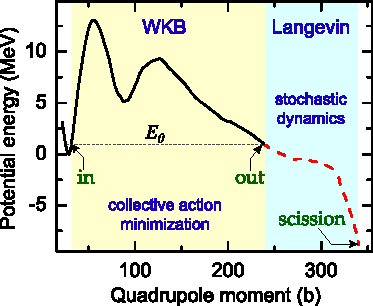
\includegraphics[width=0.5\linewidth]{TeX_files/methods_overview}
	\caption[Schematic overview of the framework for fission calculations used in this dissertation]{Schematic overview of the framework for fission calculations used in this dissertation. Source:~\cite{Sadhukhan2016}}
	\label{fig:methodsoverview}
\end{figure}

\subsection{Potential energy surfaces}
The primary degrees of freedom in the adiabatic approximation are nuclear collective shapes, and therefore the basic ingredient to fission calculations is a potential energy surface (PES). In principle, one could describe any three-dimensional shape using an infinite basis; however, for practical computations one must use a truncated set of only a few collective coordinates. Thus, an important challenge for researchers is to select the most relevant collective coordinates, ideally while demonstrating that others can be safely neglected. Often one will use the first few lowest-order multipole moments, but it should be noted that these are not always well-suited for describing shapes which occur during fission, especially near scission. One alternative was proposed in~\cite{Younes2012}. Other collective coordinates which are sometimes used in the literature include $q_N$, which controls the size of the neck, and non-geometric variables such as $\lambda_2$ or the pairing gap $\Delta$, which control pairing and pairing fluctuations.

Once the appropriate shape constraints $\vec{q}\equiv(q_1, q_2, \dots)$ are chosen, the PES is computed as a mesh: one DFT calculation per grid point. The density at each point $\vec{q}$ is then used to compute the HFB energy $E'(\vec{q})$, along with anything else which depends on the density.

\subsection{Collective inertia}
Just as important to fission dynamics as the energy of the system is the collective inertia, which describes the tendency of the system to resist configuration changes (such as shape changes). The form of the collective inertia used here is the non-perturbative adiabatic time-dependent HFB (ATDHFB) inertia with cranking~\cite{Baran2011}, which takes the form

\begin{equation}\label{eq:mATDHFB-np}
\mathsf{M}_{\mu\nu} =  \frac{\hbar^2}{2}\frac{1}{(E_a+E_b)}\left(\frac{\partial\mathcal{R}^{21}_{(0),ab}}{\partial q_\mu}\frac{\partial\mathcal{R}^{12}_{(0),ba}}{\partial q_\nu}+\frac{\partial\mathcal{R}^{12}_{(0),ab}}{\partial q_\mu}\frac{\partial\mathcal{R}^{21}_{(0),ba}}{\partial q_\mu}\right)
\end{equation}

\noindent The subscripts and superscripts are explained in the full temperature-dependent derivation of the collective inertia found in Appendix~\ref{append:TD-ATDHFB}, but the important feature to note is that computing the inertia requires differentiating the density matrix with respect to a pair of collective coordinates.

A perturbative expression for the ATDHFB inertia also exists, which allows one to estimate the inertia without taking derivatives of the density. It is computationally much faster and easier to implement, but it is less accurate and loses many of the important features of the inertia, as we shall see in Chapter~\ref{chap:294Og}. Nevertheless, it is commonly-used in calculations and later on we shall show how this choice affects fission yields compared to the non-perturbative inertia.

Another common expression for the collective inertia comes from the Generator Coordinate Method (GCM). The GCM inertia also exists in two varieties: perturbative and non-perturbative~\cite{Giuliani2018b}. Like the ATDHFB inertia, the perturbative GCM inertia is smoothed-out compared to the non-perturbative inertia. Both the perturbative and non-perturbative GCM inertias are found to be smaller in magnitude than their ATDHFB counterparts.

\subsection{WKB approximation}\label{sect:wkb}
Spontaneous fission is a form of quantum tunneling. If the wavefunction of the fissioning nucleus is assumed to be slowly-varying inside the potential barrier (which condition is satisfied under the adiabatic assumption), then the WKB approximation allows us to estimate the probability of tunneling through a classically-forbidden region in the PES.

The most-probable tunneling path $\left. L(s) \right|_{s_{\rm in}}^{s_{\rm out}}$ in the collective space is found via minimization of the collective action

\begin{equation}\label{eq:action} 
S(L) = \frac{1}{\hbar}\int_{s_{\rm in}}^{s_{\rm out}} \sqrt{2\mathcal{M}(s)\left(E'(s)-E_0\right)}ds,
\end{equation} 

\noindent where $s$ is the curvilinear coordinate along the path $L$, $\mathcal{M}(s)$ is the collective inertia given by~\cite{Sadhukhan2013}

\begin{equation}
\mathcal{M}(s) = \sum_{\mu\nu} \mathsf{M}_{\mu\nu} \frac{dq_\mu}{ds} \frac{dq_\nu}{ds}
\end{equation}

\noindent and $V(s)$ is the potential energy along $L(s)$. $E_0$ stands for the collective ground-state energy. The calculation is repeated for different outer turning points, and each of these points is then assigned an exit probability $P(s_{\rm out})=[1+\exp{2S(L)}]^{-1}$~\cite{Baran1978}. 

The half-life corresponds to the minimum action pathway, and the expression for the half-life is $T_{1/2} = \mathrm{ln}(2)/nP(s_\mathrm{min})$. The parameter $n$ is the number of assaults on the fission barrier per unit time and the standard value is $n=10^{20.38} s^{-1}$. However, because of the exponential dependence of the half-life on the action, half-life calculations are not yet reliable.

\subsection{Langevin dynamics}

Although the link between collective and intrinsic degrees of freedom was assumed away in the adiabatic approximation, it is worth reintroducing some connection between the two, especially in the region between the outer turning points and scission where the adiabatic assumption is weakest. Through the semiclassical Langevin approach~\cite{Abe1996,Frobrich1998,Sadhukhan2016}, we introduce a dissipation tensor $\eta$ that mimics energy exchange between intrinsic and collective modes. The dissipation tensor is related to a random force strength $g$ via the fluctuation-dissipation theorem, given by the expression $\sum_k g_{ik}g_{jk} = \eta_{ij}k_BT$. The fluctuation-dissipation theorem effectively couples collective and intrinsic degrees of freedom via the system temperature $T$, given by $k_BT = \sqrt{E^*/a}$ where $a=A/10$MeV$^{-1}$ parameterizes the level density and the excitation energy $E^*(\vec{q}) = E'(s_{out}) - E'(\vec{q}) - \frac{1}{2}\sum\left(\mathcal{M}^{-1}\right)_{ij}p_i p_j$.

After emerging from the classically-forbidden region of the PES, fission trajectories continue across the PES from the outer turning line, evolving according to the Langevin equations:
\begin{gather}\label{eq:langevin} 
	\frac{dp_i}{dt} =  
	-\frac{p_j p_k}{2} \frac{\partial}{\partial q_i}\left(\mathcal{M}^{-1}\right)_{jk} 
	- \frac{\partial E'}{\partial q_i}  - \eta_{ij}\left(\mathcal{M}^{-1}\right)_{jk} p_k + g_{ij}\Gamma_j(t) \,, \\ 
	\frac{dq_i}{dt} = 	\left(\mathcal{M}^{-1}\right)_{ij} p_j \,,  
\end{gather} 
\noindent where $p_i$ is the collective momentum conjugate to $q_i$, and $\Gamma_j(t)$ is a Gaussian-distributed, time-dependent stochastic variable. From here one can see that the dissipation term\\\noindent $- \eta_{ij}\left(\mathcal{M}^{-1}\right)_{jk} p_k$ represents a transfer of energy away from the collective motion of the system, while the random fluctuation term $g_{ij}\Gamma_j(t)$ does the opposite.

Dissipation is treated in our work as a parameter, as a self-consistent description of dissipation is not yet known.  In the meantime, we use the values from~\cite{Sadhukhan2016}, which were fitted to reproduce the $^{240}$Pu fragment yields.% However, work along this line has been started (maybe?) in refs 291-293 of~\cite{Schmidt2018} (see Section 4.1.1 for the context).

\subsection{Localization plus Grand Canonical Ensemble}\label{sect:loc-frags}
The Langevin approach represents the best of what static approaches currently have to offer in terms of quantitative reproduction of the yields; however, it can be expensive and time-consuming to perform a full Langevin calculation with non-perturbative collective inertia in a multidimensional collective space. For applications where the level of quantitative accuracy is somewhat flexible (an example would be r-process network calculations, which are explained in Chapter~\ref{chap:rprocess}), is it necessary to do all these calculations? Or is there some kind of physical insight that can be leveraged to reduce the workload?

By studying nucleon localization functions (Section~\ref{sect:locali}) for deformed configurations of several fissioning nuclei, we observe that, in many cases, two distinct fragments start to form independently and then separate well before scission is reached. Thus, a fissioning nucleus can be thought of as two well-formed prefragments connected by a neck. At scission, the two prefragments separate and the remaining neck nucleons are distributed to either of the two prefragments in some predictable way.

Based on this, we created the following prescription for identifying prefragments and estimating fragment yields at the outer turning line:

\begin{itemize}
	\item Identify possible prefragments using the density and nucleon localization function (see Figure~\ref{fig:methods240Pulocali}):
		\subitem Along the primary axis of the nucleus, find the two locations (one for each fragment) at which the density is widest. This is taken to be the approximate center of each fragment.
		\subitem For each fragment, start from the central value and locate the two nearest optima in the localization (maximum or minimum; one on either side). This gives you a range of possible central values.
		\subitem Sum up the nucleons above (below) the central value and multiply by two to determine the identity of the upper (lower) prefragment.
	\item The remaining neck nucleons are assumed to form into clusters: alpha particles first, then a deuteron if there is one of each nucleon left, plus some remaining free protons or neutrons.
	\item The total binding energy of the prefragments and any particles/clusters is subtracted from the total energy of the system to get the energy of the neck, $E_{neck}$.
		\subitem Use this energy to define the temperature of the system: $T = \sqrt{\left|E_{neck}/a\right|}$ where the level density parameter $a$ we take to be $a=A_p/10$ MeV$^{-1}$ with $A_p$ the mass number of the parent nucleus.
	\item Use brute force combinatorics to find every possible way of assigning the neck particles to either of the prefragments (including the possibility that a particle/cluster might be emitted instead of flowing to a prefragment).
	\item For each fragments + particles combination, look up the binding energy of each of the final fragments in a table (such as  MassExplorer \verb|\cite{???}|).
	\item The Coulomb repulsion energy between the fragments plus the total binding energy of the fragments and any remaining clusters is subtracted from the total energy of the system to get the residual (kinetic + intrinsic) energy, $E_{res}$.
	\item I use this energy to define the a grand canonical ensemble (note that the chemical potentials are hidden in the binding energies): $Z = \sum e^{-\frac{E_{res}}{k_BT}}$
	\item Calculate probabilities: $P(n_1,z_1,n_2,z_2) = \frac{1}{Z} e^{-\frac{E_{res}(n_1,z_1,n_2,z_2)}{k_BT}}$
	\item [I convoluted those probabilities with a Gaussian, as we did in the paper.]
\end{itemize}

\begin{figure}
	\centering
	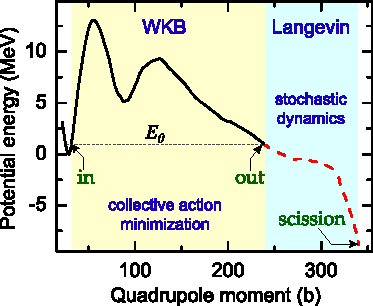
\includegraphics[width=0.5\linewidth]{TeX_files/methods_overview}
	\caption[Localization function for 240Pu with lines drawn to represent prefragment identification]{Localization function for 240Pu with lines drawn to represent prefragment identification}
	\label{fig:methods240Pulocali}
\end{figure}

The fact that this can be estimated at the outer turning line instead of at scission is a tremendous reduction in the number of PES points which must be computed. Furthermore, our experience with the WKB approximation shows that most trajectories leading to the outer turning line actually follow the minimum action path, branching away only just before reaching the outer turning line. In Chapter~\ref{chap:rprocess}, we will compute a 1-dimensional PES between the ground state and the outer turning line (either the static path or the minimum action path), and a 2-dimensional PES in the region of the outer turning line. This is a substantial reduction compared to the Langevin calculations, but the $^{240}$Pu SF yields shown in Figure~\ref{fig:methods240Puyield} are similar, with similar peaks and widths, but with appropriately wider uncertainty bands for the localization + grand canonical ensemble method.

\begin{figure}
	\centering
	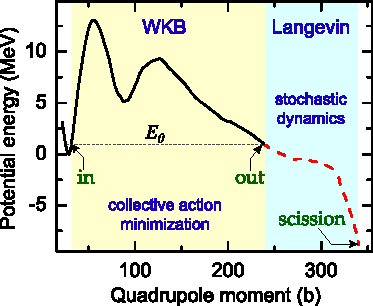
\includegraphics[width=0.5\linewidth]{TeX_files/methods_overview}
	\caption[Computed spontaneous fission yields for 240Pu compared to experimental data. The Langevin yields are shown in ??? color and are taken from~\cite{Sadhukhan2016}. The localization yields are shown in ??? color. Experimental data is shown in ??? color and comes from ??? source.]{Computed spontaneous fission yields for 240Pu compared to experimental data. The Langevin yields are shown in ??? color and are taken from~\cite{Sadhukhan2016}. The localization yields are shown in ??? color. Experimental data is shown in ??? color and comes from ??? source.}
	\label{fig:methods240Puyield}
\end{figure}